\section{Photo originale}\label{photo-originale}

\emph{Toutes les comparaisons sont faites avec la photo originale.}

\begin{figure}[htbp]
\centering
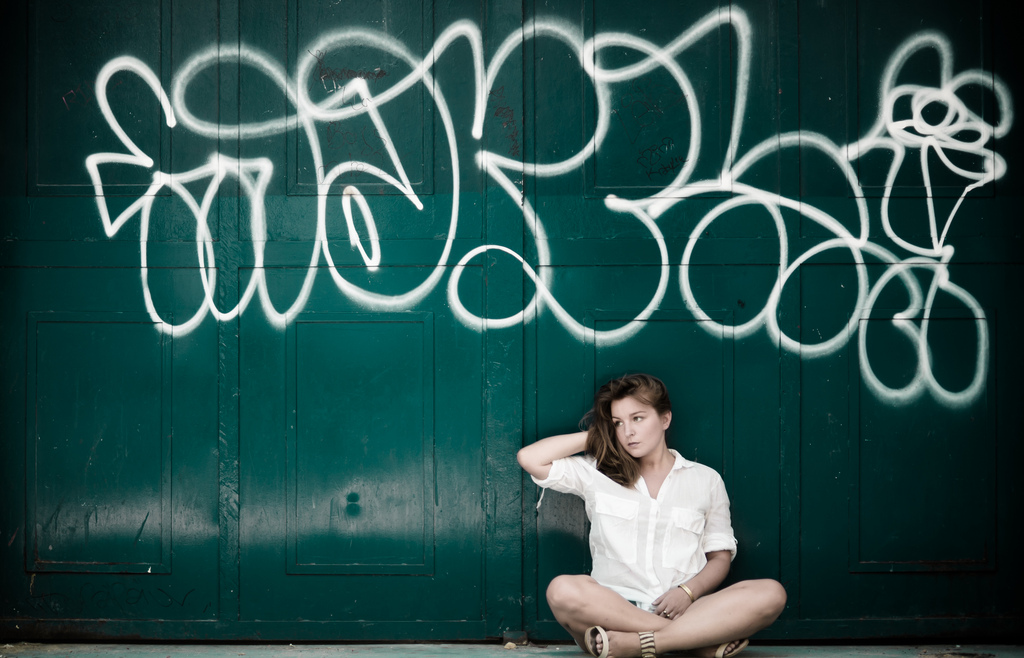
\includegraphics{../../photos/original.jpg}
\caption{Photo original}
\end{figure}

Pour les comparaisons, nous utilisons deux procédés :

\begin{description}
\item[La distance de Bhattacharyya] qui est une mesure de la similarité de deux
  distributions de probabilités discrètes. On la calcule après création
  d'histogrammes pour chaque text = Image.
\item[Le filtre de Sobel] qui permet une détection des contours. Nous comparons
  ensuite les deux text = Images créées avec le filtre de Sobel pixel à pixel pour
  avoir une comparaison des contours et donc des formes présentes sur la photo.
\end{description}